\documentclass[conference]{IEEEtran}

\usepackage{setspace}
\usepackage{mathrsfs}
\usepackage{amsmath}
\usepackage{amsfonts}
\usepackage{amsthm}
\usepackage{amssymb}
\usepackage{graphicx}
\usepackage{subfigure}
\usepackage{indentfirst}
\usepackage{array}
\usepackage{cite}
\usepackage{enumerate}
\usepackage[linesnumbered,ruled,vlined]{algorithm2e}
\usepackage{multirow}
\usepackage{verbatim}
\usepackage{stfloats}
\usepackage{color}
\newtheorem{theorem}{\bf{Theorem}}
\newtheorem{lemma}{\bf{Lemma}}
\newtheorem{proposition}{\bf{Proposition}}
\newtheorem{corollary}{\bf{Corollary}}
\newtheorem{conjecture}{\bf{Conjecture}}
\newtheorem{definition}{\bf{Definition}}
\newtheorem{remark}{\bf{Remark}}

\hyphenation{location-based}

\begin{document}
\title{Improved DetNet for MIMO Detection}

\author{\IEEEauthorblockN{Guili Gao, Chao Dong, Kai Niu}
\IEEEauthorblockA{Key Laboratory of Universal Wireless Communications, Ministry of Education\\
Beijing University of Posts and Telecommunications, Beijing, China 100876\\
Email: \{2016140061, dongchao, niukai\}@bupt.edu.cn}
}

\maketitle
\begin{abstract}
In this paper, we refer DetNet\cite{DetNet}'s design, simplify the network structure of DetNet, reduce complexity from 8n*8n to 3n, and improve performance.

\end{abstract}

\IEEEpeerreviewmaketitle

\section{Introduction}
Multiple-input multiple-output system can improve the throughput of the network, improve the communication quality, achieve multiple reception with multiple antennas, and increase the channel capacity by several times without increasing the spectrum resources and the antenna transmission power, Advantages, has been applied to most communication systems. However, the complexity of signal detection in MIMO system is very high at present. Commonly used traditional detection methods fall into two categories: linear detection and nonlinear detection; linear detection includes ZF and MMSE; nonlinear detection methods are AMP, SDR and ML; Although the detection of low complexity, but poor performance; non-linear detection performance is better, but the complexity is high. In recent years, the research on machine learning has become a global hot spot. While studying and learning, we learned to adopt DetNet to solve the problem of MIMO detection. After further study, there are several points in this network to improve the network In this paper, we propose a method to simplify the network, which can improve the performance of the network while reducing the network complexity.

With the potential large gains in spectral efficiency and energy efficiency, massive MIMO is a promising technology that the next generation of wireless systems may incorporate\cite{MIMO1}. The key problem with Massive MIMO is to design a low-complexity detector with good performance. The complexity of the detector is exponential as the number of antennas increases. Therefore, it is very important to reduce the complexity of the detector to the scene with a large number of antennas. The optimal detection scheme is the maximum likelihood(ML) detection, but it has the highest computational complexity. To reduce computational complexity, the linear detector is used for MIMO detection. such as minimum mean squared error (MMSE) and zero-forcing (ZF) detectors \cite{MIMO2}. but the performance of linear detection is poor. There are other suboptimal algorithms, including approximate
message passing (AMP) and semidefinite relaxation (SDR)\cite{problem}, \cite{detector}. Both AMP and SDRS are near-optimal performance algorithms in actual scenarios.

In the past few decades, machine learning has been a great success in many fields, and we have witnessed the process from being put forward to application. There are many algorithms in machine learning, we choose suitable model algorithm according to the different characteristics, supervised learning, linear regression, decision tree, neural network and SVM, most got the learning algorithm, and unsupervised learning represented by cluster analysis. The prediction of discrete values of data is called classification. Called for the forecast of successive regression, the training model, existing data sets will be divided into training set and test set, the training set is used to model of training, testing machine is used to model ability assessment.
The most rapid development in recent years is deep learning, especially in image processing and artificial intelligence, Deep learning is a multi-layer neural network constructed by complex connections, and the network connection structure is adjusted according to different application scenarios. When training program, the data of the output layer gradient calculation, and then to back propagation, according to the gradient change network weights, make the output results are closer to the ideal, but with the increase of network layer, training time will increase, and the gradient will radiate or disappear. To some extent, ResNet\cite{ResNet} can reduce the number of layers in the network, increase the speed of convergence, and improve the performance. ResNet is referenced in the network structure of this paper.
Deep learning is one of the most active areas of machine learning. Deep learning begin to gradually applied in the wireless communication field, including in the field of channel coding, for LDPC code, using the relationship between check nodes and variable nodes, designed based on the Belief propagation deep learning network\cite{BCH}��Based on this design, the network can accelerate the convergence speed of the traditional BP network, and the performance will not lose, and even surpass the traditional network. For the end-to-end system, the autoencoder can be abstracted; CsiNet\cite{feedback} can be used to compress and decompress the feedback of downlink channel information to base station.

DetNet is the depth of a multilayer neural network, dedicated to channel detection, when the sender send multiple symbols after the fast fading channel, gaussian white noise, multiple antennas at the receiving end will receive a signal input into the trained DetNet, after DetNet output, are the result of the test. After verification, the performance of DetNet is much higher than that of MMSE and ZF when the number of lines is increased, and it can approach the performance of AMP algorithm. The use of DetNet is divided into two phases, the training phase and the use phase. When training, specify the number of antennas and receiving antennas, and the number of nodes in the network is determined; Each group of training data will undergo different fast fading channels and different signal-to-noise ratio. The receiver will input these signals into the network for training, and the training will be followed by the backward propagation algorithm. In use phase, the network has been trained, in this stage, to adjust the network weights is no longer, after training the network can be applied to different fast fading channel, than a different channel. The following are the advantages and disadvantages of DetNet.
\begin{itemize}
\item Advantage:
    \begin{enumerate}
        \item  The performance of DetNet is similar to the performance of suboptimal algorithm, and with the increase of the number of antennas, the performance is better and better.
        \item  DetNet has good robustness and can adapt to different SNR and different channels.
        \item  The structure of DetNet can be processed in parallel.
    \end{enumerate}
\item Disadvantages:
    \begin{enumerate}
        \item  When the number of antennas is relatively small, the performance is worse than that of linear detection.
        \item  DetNet requires that the sender has fewer antennas than the receiving end, and if the number of antennas is close or the number of antennas is larger than the number of receiving antennas, the performance will be poor.
    \end{enumerate}
\end{itemize}

The contribution of this paper can be summarized as follows.

In this paper, we define the channel matrix as \textbf{H},the transmit vector as \textbf{x}, and the receive vector as \textbf{y}, Boldface uppercase letters denote matrices, Boldface lowercase letters denote vectors, the superscript ${(\centerdot)^T}$ denotes the transpose.

\section{System Model}
In this section, we will introduce in detail the traditional method of MIMO detection, and then introduce the process of DetNet from traditional detection to DetNet framework.
\subsection{MIMO Detection}
For a MIMO system, we assume that it contains n transmit antennas, m receive antennas, and n <m. The data stream is serialized and converted into n parallel spatial data substreams. Using BPSK modulation, sent through the n antenna to send out, through the wireless channel to the receiving end, the system model can be expressed as:

\begin{equation}
\label{basic model}
\textbf{y}=\textbf{Hx}+\textbf{w}
\end{equation}

Where \textbf{y} is a vector of ${m \times 1}$ dimensions, \textbf{x} is a vector of ${n \times 1}$ dimensions, \textbf{w} is a ${m \times 1}$ independent, zero-mean Gaussian white noise vector and H is ${m \times n}$ the fading channel model of the matrix.

Our goal is to derive the transmitted signal \textbf{x} from the received \textbf{y}; This problem can be solved by maximum likelihood(ML) detection. ML detection can ensure the minimum detection error rate. The ML detection searches for the transmitted signal vector \textbf{x} by exhaustive search and calculates the Euclidean distance between the received signal vectors \textbf{y} and \textbf{Hx} , And then select the value from the received signal vector \textbf{y} Euclidean distance \textbf{x}��
\begin{equation}
\label{ML}
\hat{x}=\mathop{\arg\min}_{x\in\{\pm1\}^K}\|\textbf{y-Hx}\|^2
\end{equation}
ML detection theoretically achieves the best performance, but as the number of transmit antennas increases, the complexity increases exponentially, which is impractical for large-scale MIMO and is therefore rarely used in practical systems Detection.


\subsection{DetNet}
DetNet was proposed by Neev Samuel, it is a multi-layer neural network dedicated to MIMO detection, the overall structure of the network is as Fig.\ref{Network model}.
\begin{figure}[ht]
  \centering
  \includegraphics[width=0.5\textwidth]{DetNetFormWork.pdf}
  \caption{DetNet Formwork}
  \label{Network model}
\end{figure}
Each unit has the same structure and contains four inputs: ${\textbf{H}^T\textbf{y}}$, ${\textbf{H}^T\textbf{H}}$, \textbf{x} and \textbf{v}, where${\textbf{H}^T\textbf{y}}$ and ${\textbf{H}^T\textbf{H}}$ are the common inputs for each unit, and they are the same for each set of transmitted sequences, while \textbf{x} and \textbf{v}, for each unit are different; we can be seen from the figure the entire network structure also introduces a residual network form, that is the next unit of input \textbf{x} and \textbf{v}, equal to the output of this unit plus the previous unit��s input, used to speed up the network convergence speed and improve performance;
\begin{equation}
\label{ResNet}
\begin{split}
&{\textbf{x}_{in}^l}=\mu{\textbf{x}_{out}^{l-1}}+(1-\mu)\textbf{x}_{in}^{l-1}\\
&{\textbf{v}_{in}^l}=\mu{\textbf{v}_{out}^{l-1}}+(1-\mu)\textbf{v}_{in}^{l-1}
\end{split}
\end{equation}


$\mu$  is a residual coefficient, Through the iteration of this multi-layer network structure, the output of each layer network can be gradually approached to the transmission vector; for this feature, it can be expressed as:
\begin{equation}
\label{DetNetTheory}
\begin{split}
\textbf{x}_{in}^{l+1} &=\prod\left[\textbf{x}_{in}^{l}-\delta_l\left.\frac{\partial\|\textbf{y}-\textbf{Hx}\|^2}{\partial\textbf{x}}\right|_{\textbf{x}=\textbf{x}_{in}^l}\right]\\
&=\prod\left[\textbf{x}_{in}^l-2\delta_l\textbf{H}^T\textbf{y}+2\delta_l\textbf{H}^T\textbf{Hx}_l\right]
\end{split}
\end{equation}
${\textbf{x}_{in}^l}$ is the estimated signal of layer $l-1$ and $\delta_l$ is the learning rate. Thus, the output ${\textbf{x}_{out}^l}$ of each layer is gradually approaching the sending signal \textbf{x}.
It can be seen from formula $\left(\ref{DetNetTheory}\right)$ that the performance of the network is related to \textbf{Hy} and ${\textbf{H}^T\textbf{Hx}}$ only, meanwhile adding \textbf{v} to the input as the input of each layer network.

Fig.\ref{DetNet unit} is the structure of each unit, First, it concatenates the inputs and then extends the concatenation of the vectors to higher dimensions and finally to the dimensions of \textbf{x} and \textbf{v}.

\begin{figure}[ht]
  \centering
  \includegraphics[width=0.5\textwidth]{DetNet.pdf}
  \caption{DetNet}
  \label{DetNet unit}
\end{figure}

The dimension of ${\textbf{H}^T\textbf{y}}$ is ${n \times 1}$, the dimension of v is ${2n \times 1}$, the dimension of x is ${n \times 1}$, the dimension of ${\textbf{H}^T\textbf{H}}$ is ${n \times n}$, ${W_{1k}, W_{2k}, W_{3k}, b_{1k}, b_{2k}, b_{3k}}$ is the network weight to train. After operation CONCAT, the vector dimension output from CONCAT is ${5n \times 1}$, the operation after CONCAT is to transform the CONCAT outputs through a layer of fully connected network into high dimension, $\rho$ is sigmod function as activation Function, then the output of $\rho$ input to a layer of network for compression to \textbf{v} and \textbf{x} dimensions, and then output separately, wherein the output is compressed into the \textbf{x} dimension, Since the final \textbf{x}${\in\{\pm1\}^K}$, the activation function used is similar to function $tanh$ whose formula is
\begin{equation}
\label{twoValueFunction}
\Psi_{t\left(x\right)}=-1+\frac{\rho\left(x+t\right)}{|t|}-\frac{\rho\left(x-t\right)}{|t|}
\end{equation}
The maximum value of this function is 1, the minimum is -1.The above is a unit network structure, each unit will be cascaded to form the entire network. The number of unit is 90.
The loss function of the network is
\begin{equation}
\label{lossFunction}
Loss=\sum_{l=1}^L\log\left(k\right)\frac{\|\textbf{x}-\hat{\textbf{x}}_k\|^2}{\|\textbf{x}-\widetilde{\textbf{x}}_k\|^2}
\end{equation}
where:
\begin{equation}
\label{lossFunction}
\widetilde{\textbf{x}}=\left(\textbf{H}^T\textbf{H}\right)^{-1}\textbf{H}^T\textbf{y}
\end{equation}
The performance of DetNet can be referenced \cite{DetNet}.

\section{Improved DetNet}
Although DetNet is a good performance MIMO detection neural network, we still find there are still some improvements, we call the improved net 'NfdNet';
We take ${2 \times 2}$ MIMO structure as an example, expand Fig.\ref{DetNet unit} into the form of network node,as shown in Fig.\ref{DetNetConnect}. The input of a node in Fig.\ref{DetNetConnect} represents an element of a vector.
\begin{figure}[ht]
  \centering
  \includegraphics[width=0.4\textwidth]{DetNetConnect.pdf}
  \caption{DetNet Network Connection}
  \label{DetNetConnect}
\end{figure}
\subsubsection{Remove Input \textbf{v}} It can be seen that although \textbf{x} and \textbf{v} are separate, it can be seen that we are only using a fraction of the total output for the true approximation of the transmitted signal, where as the part belonging to \textbf{v} does not provide any information to the network, just as a The amount of filling, its role is similar to the role of network bias, and the addition of \textbf{v}, for each unit have increased a large number of connection changes, increasing the complexity of the network, for the entire network, the removal of \textbf{v} can be substantial simplify the network structure. Before removing \textbf{v}, the number of edges per unit is ${8n \times 8n}$, the number of edges after removing \textbf{v} is ${4n \times 8n}$, the total connection variable is reduced by half and the training parameters are reduced by half. After removing \textbf{v}, the network is shown in figure Fig.\ref{DetNetRemoveV}.
\begin{figure}[ht]
  \centering
  \includegraphics[width=0.4\textwidth]{DetNetRemoveV.pdf}
  \caption{DetNet Network Remove \textbf{v}}
  \label{DetNetRemoveV}
\end{figure}
\subsubsection{Simplified Network Connection} After removing the \textbf{v}, the network nodes are still using a fully connected structure, for each input node information,it needs to interact with other nodes, but from Equation \(\ref{DetNetTheory}\), it can be seen that the nodes in the network actually interact with each other between ${\textbf{H}^T\textbf{y}, \textbf{x}_{\texttt{in}}^l, \textbf{H}^T\textbf{Hx}_{\texttt{in}}^l}$, for other nodes information is not required to interact. Fig.\ref{NfdNet} is a simplified unit network structure diagram,It is not fully connected detection network(NfdNet). In NfdNet, the first node of each vector is only connected with the output of the first node, the second node only with the output of the second node connected, and so on.
\begin{figure}[ht]
  \centering
  \includegraphics[width=0.3\textwidth]{NfdNet.pdf}
  \caption{neural network connection for NfdNet}
  \label{NfdNet}
\end{figure}
Before simplification, the number of edges of each unit is ${8n \times 8n}$. After removing \textbf{v} and simplifying the network connection, the number of connected edges of the network is only ${3n}$.
\subsubsection{Simplified Loss Function} The loss function for DetNet is as follows:
\begin{equation}
\label{NfdNetLoss}
Loss=\sum_{l=1}^L\log\left(k\right)\|\textbf{x}-\hat{\textbf{x}}_k\|^2
\end{equation}
Our loss function removes ${\|\textbf{x}-\left(\textbf{H}^T\textbf{H}\right)^{-1}\textbf{H}^T\textbf{y}\|^2}$ compared to DetNet's loss function. Actually this formula is equivalent to  ${\|\textbf{w}\|^2}$. Our goal is to make estimates of the output and send signals are equal, therefore, we remove the formula, another reason that we remove this formula is: this formula contains inversion operation, in many cases, the square matrix is not reversible. After our tests found that this formula was removed, the performance improved slightly.
In our simulation, after the output of the last layer passes through the $\Psi$ activation function, the range will be ${\textbf{y}\in\left(1,-1\right)}$, we judge the results by
\begin{equation}
\textbf{y}_{\textrm{out}}=\left\{
\begin{aligned}
&1  &\mbox{${\textbf{y}_{\textrm{out}}^N\geqslant0}$}\\
&0  &\mbox{${\textbf{y}_{\textrm{out}}^N<0}$}
\end{aligned}
\right.
\end{equation}

In this section, inspired by DetNet, we propose a simplified deep learning model for MIMO detection. In the following sections, we will compare the performance of these two networks.

\section{Simulation Results}

In this section, we will compare the performance of DetNet and NfdNet, the following is the simulation conditions:
all simulation channels are on fast fading channels, and the channel ratio of each simulation is immediately chosen in the range of [7, 14]. In DetNet, the dimension of \textbf{v} is ${2 \times m}$, the extended dimension from inputs is ${8 \times m}$ and the learning rate is 0.0001.
\begin{figure}[ht]
  \centering
  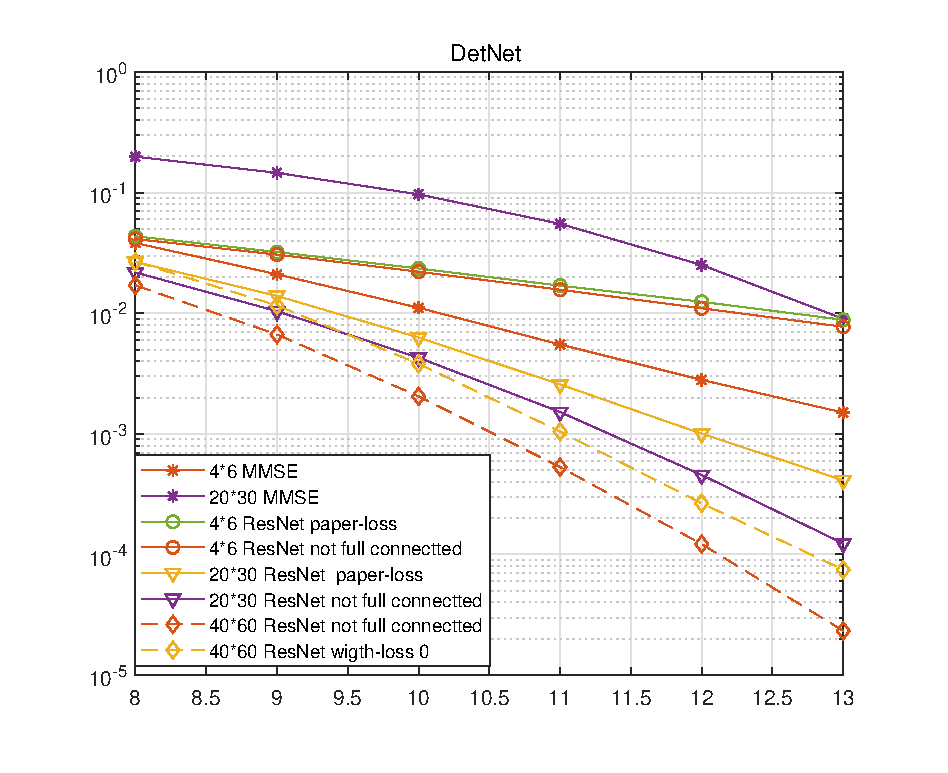
\includegraphics[width=0.5\textwidth]{beforeResult.eps}
  \caption{neural network connection for NfdNet}
  \label{NfdNet1}
\end{figure}


\section{Conclusions and Future Work}
In this paper, we proposed a cross-layer improved GPSR

\section*{Acknowledgement}
This work is supported by the National Natural Science Foundation of China (No. 61671080) and Huawei Corporation.


\begin{thebibliography}{99}
\bibitem{DetNet}
N. Samuel, T. Diskin and A. Wiesel, "Deep MIMO detection," \emph{2017 IEEE 18th International Workshop on Signal Processing Advances in Wireless Communications (SPAWC)}, Sapporo, 2017, pp. 1-5. doi: 10.1109/SPAWC.2017.8227772

\bibitem{MIMO1}
F. Rusek, D. Persson, B. K. Lau, E. G. Larsson, T. L. Marzetta,O. Edfors, and F. Tufvesson, “Scaling up mimo: Opportunities and challenges with very large arrays”, \emph{IEEE Signal Processing Magazine}, vol. 30, no. 1, pp. 40~C60, 2013.

\bibitem{MIMO2}
S. Yang and L. Hanzo, “Fifty years of mimo detection: The road to large-scale mimos”,\emph{IEEE Communications Surveys \& Tutorials}, vol. 17, no. 4, pp. 1941~1988, 2015.

\bibitem{problem}
Z. Q. Luo, W. K. Ma, A. M. So, Y. Ye, and S. Zhang, “Semidefinite relaxation of quadratic optimization problems”, \emph{IEEE Signal Processing Magazine}, vol. 27, no. 3, pp. 20~C34, 2010

\bibitem{detector}
J. Jalden and B. Ottersten, “The diversity order of the semidefinite relaxation detector”, \emph{IEEE Transactions on Information Theory}, vol. 54, no. 4, pp. 1406~C1422, 2008.

\bibitem{ResNet}
K. He X. Zhang S. Ren J. Sun "Deep Residual Learning for Image Recognition" in \emph{Computer Vision and Pattern Recognition IEEE} pp. 770-778 2016.

\bibitem{BCH}
E. Nachmani, Y. Be'ery and D. Burshtein, "Learning to decode linear codes using deep learning" \emph{2016 54th Annual Allerton Conference on Communication, Control, and Computing (Allerton)}, Monticello, IL, 2016, pp. 341-346.

\bibitem{feedback}
C. K. Wen, W. T. Shih, S. Jin “Deep Learning for Massive MIMO CSI Feedback” arXiv preprint arXiv: 1712.08919, 2017.

\end{thebibliography}

\end{document}
